\documentclass[10pt,utf8]{beamer}

\mode<presentation> {
  \usetheme{Madrid}
  \setbeamercovered{transparent}
}

\usepackage{palatino}
\usepackage{graphicx}
\usepackage{array}
\usepackage{color}
\usepackage{subfigure}
\usepackage{colortbl}
\usepackage{amsmath}
\usepackage{hyperref}
\usepackage{listings}
\usepackage{fancyvrb}
\usepackage[export]{adjustbox}
%\usepackage{tikz}
%\usetikzlibrary{arrows,shapes,backgrounds}


\definecolor{MyDarkGreen}{rgb}{0.3,0.7,0.3}

\setbeamertemplate{caption}{\raggedright\insertcaption\par} %turn off caption prefix ("Figure")

\title{Building distributed machine learning pipeline}
\author{Vojtěch Juránek}
\institute[Red Hat]{JBoss - a division by Red Hat}
\date{27.~1.~2017, DEVCONF.CZ, Brno}

\newenvironment{mylisting}
{\begin{list}{}{\setlength{\leftmargin}{1em}}\item\scriptsize\bfseries}
{\end{list}}

\newenvironment{mytinylisting}
{\begin{list}{}{\setlength{\leftmargin}{1em}}\item\tiny\bfseries}
{\end{list}}

% see http://tex.stackexchange.com/questions/151254/coloring-or-bolding-multiple-lines-in-fancyvrb-integration-with-listings
\lstdefinestyle{Java}{
	basicstyle          = \small\ttfamily,
	language            = Java,
	numbers             = left,
	numberstyle         = \tiny,
	stepnumber          = 1,
	numbersep           = 5pt,
	backgroundcolor     = \color{white},
	showspaces          = false,
	showstringspaces    = false,
	showtabs            = false,
	frame               = single,
	tabsize             = 2,
	captionpos          = b,
	breaklines          = true,
	breakatwhitespace   = false,
	morestring          = [b]",
	stringstyle         = \color{blue},
	keywordstyle        = \color{magenta},
	commentstyle        = \color{gray},
	identifierstyle     = \color{black},
	moredelim           = **[is][\bfseries]{`}{`},
	moredelim           = **[is][\color{gray}]{|}{|}, %Scala style not available, mark keyworkds by hand
	fancyvrb            = true,
}

\lstdefinestyle{Python}{
	basicstyle          = \small\ttfamily,
	language            = Python,
	numbers             = left,
	numberstyle         = \tiny,
	stepnumber          = 1,
	numbersep           = 5pt,
	backgroundcolor     = \color{white},
	showspaces          = false,
	showstringspaces    = false,
	showtabs            = false,
	frame               = single,
	tabsize             = 2,
	captionpos          = b,
	breaklines          = true,
	breakatwhitespace   = false,
	morestring          = [b]",
	stringstyle         = \color{blue},
	keywordstyle        = \color{magenta},
	commentstyle        = \color{gray},
	identifierstyle     = \color{black},
	moredelim           = **[is][\bfseries]{`}{`},
	moredelim           = **[is][\color{gray}]{|}{|},
	fancyvrb            = true,
}

\lstdefinestyle{XML}{
	basicstyle          = \small\ttfamily,
	language            = Xml,
	numbers             = left,
	numberstyle         = \tiny,
	stepnumber          = 1,
	numbersep           = 5pt,
	backgroundcolor     = \color{white},
	showspaces          = false,
	showstringspaces    = false,
	showtabs            = false,
	frame               = single,
	tabsize             = 2,
	captionpos          = b,
	breaklines          = true,
	breakatwhitespace   = false,
	morestring          = [b]",
	stringstyle         = \color{blue},
	keywordstyle        = \color{magenta},
	commentstyle        = \color{gray},
	identifierstyle     = \color{black},
	moredelim           = **[is][\bfseries]{`}{`},
	moredelim           = **[is][\color{gray}]{|}{|},
	fancyvrb            = true,
}

\begin{document}
	
\begin{frame}
 \titlepage
\end{frame}
	
\begin{frame}
	\frametitle{Data today}
	\begin{figure}
		\centering
		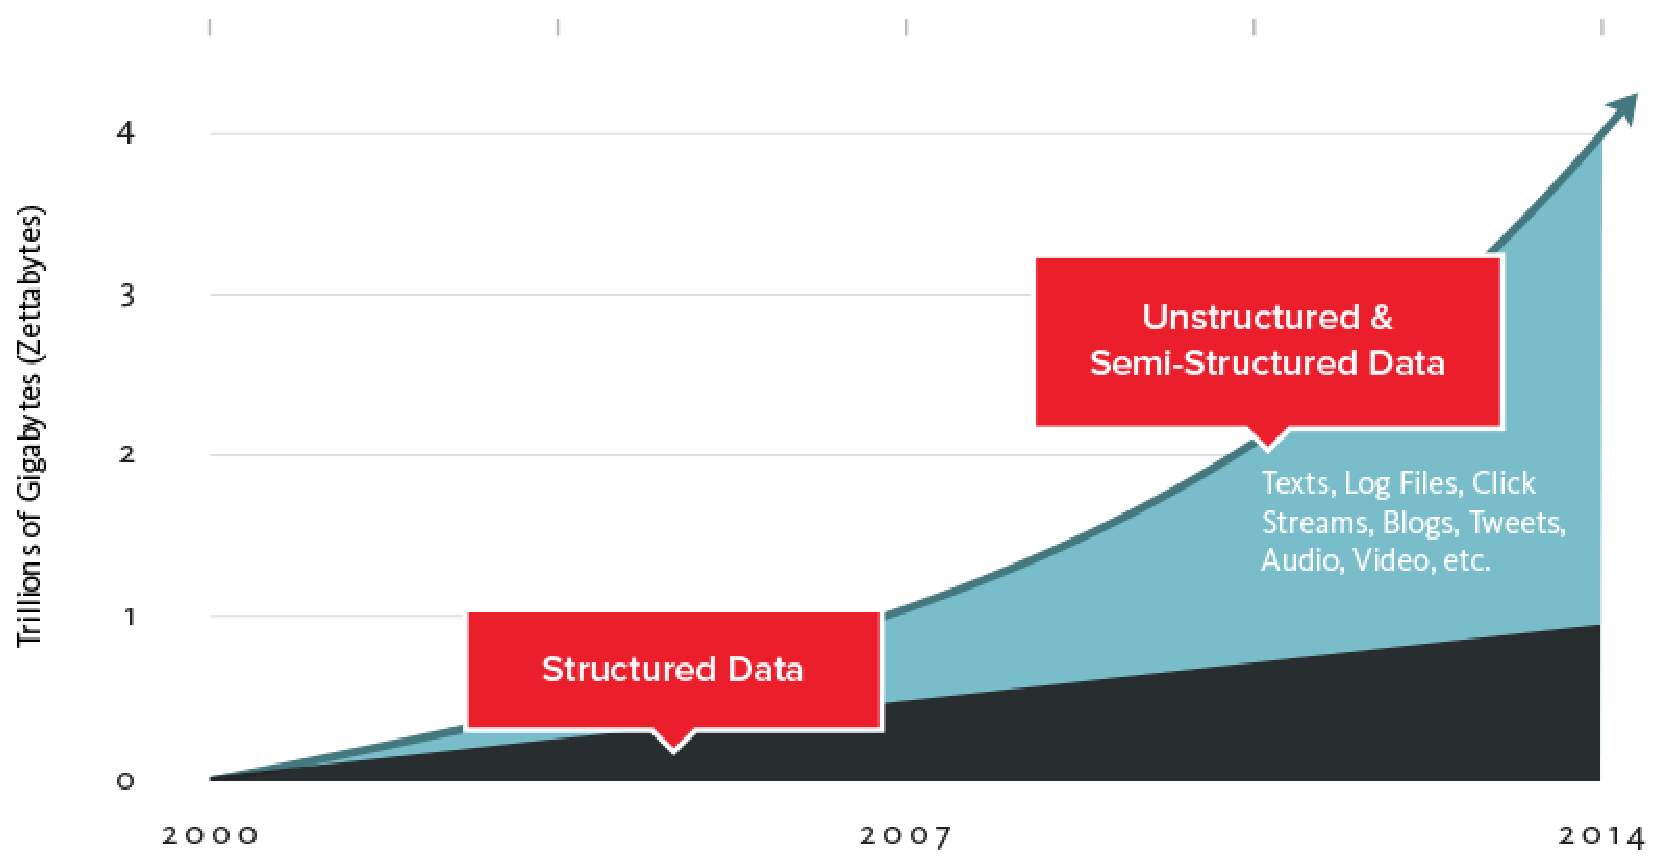
\includegraphics[width=10cm]{./img/why-nosql-2.eps}
		\caption{\tiny{Source: \url{http://www.couchbase.com/nosql-resources/what-is-no-sql}}}
	\end{figure}
\end{frame}

\begin{frame}
	\frametitle{Dealing with unstructured data}
	\begin{itemize}
		\item There are classes of problems where simple (e.g. linear) models work fine, but there are also classes there liner models fail.
% 	 \item In many cases simple models work fine.
% 	 \pause
% 	 \item Apache Spark is very usefull and popular tool for many kinds of problems.
% 	 \pause
% 	 \item But what to do when youo needs some complicated and non-liner models?
	\end{itemize}
\end{frame}

\begin{frame}
	\frametitle{Deep learning}
% 	\begin{itemize}
% 		\item \color{red}Warning: buzzword detected!\color{black}
% 		\pause
% 		\item Simply put: re-invention of neural networks (NN), more specifically deep neural networks.
% 		\pause
% 		\item Became popular in past couple of year as prices of CPU and GPU decreased.
% 		\pause
% 		\item Deep neural networks - NN with 2 or more hidden layers.
% 	\end{itemize}
% 	\visible<4> {
	\visible<2> {
		\begin{figure}
			\centering
			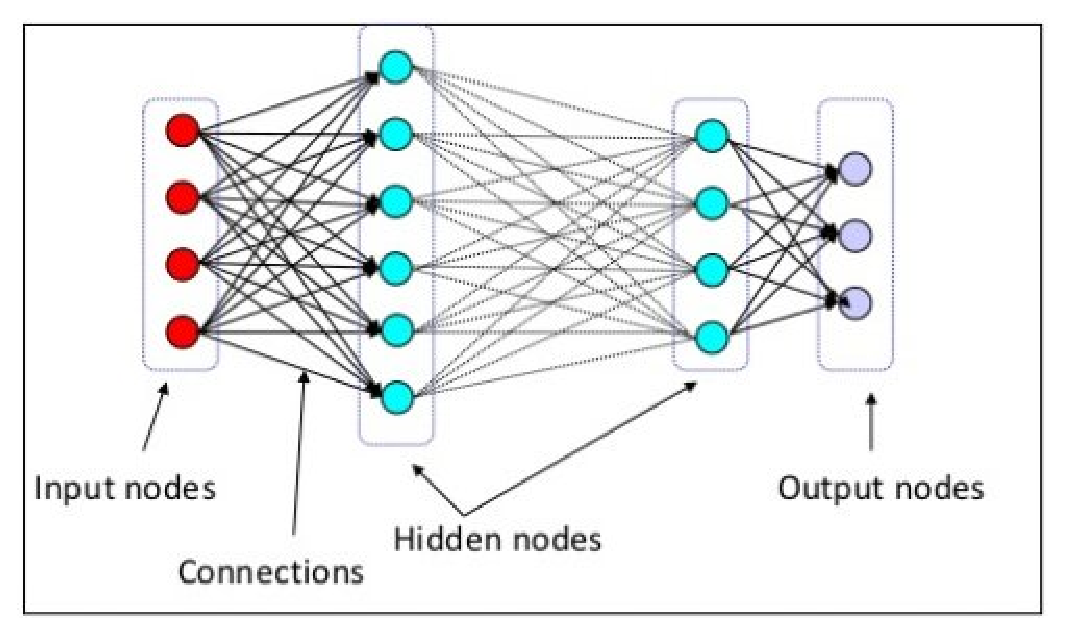
\includegraphics[width=8cm]{./img/neural-networks-layers.eps}
			\caption{\tiny{Source: \url{http://www.kdnuggets.com/2016/10/deep-learning-key-terms-explained.html}}}
		\end{figure}
	}
	%}
\end{frame}

\begin{frame}
	\frametitle{Big Data $\rightarrow$ Fast Data}
	\begin{itemize}
		\item Pressure to react/process data immediately as it arrives, provide user immediate feedback.
		\pause
		\item Big Data $\rightarrow$ Fast Data
	\end{itemize}

	\vspace{1cm}
	
	\visible<3,4,5,6> {
		\begin{itemize}
			\pause
			\item Process data once it arrives (data/event streaming).
			\pause
			\item Do the data analysis with frameworks which keep the data in memory during processing.
			\pause
			\item If possible, keep data in memory during whole application stack.
			\pause
			\item More in my DevConf 2016 \color{blue}\href{https://www.youtube.com/watch?v=98zYYs7c2wc}{talk}\color{black}~(\color{blue}\href{https://github.com/vjuranek/presentations/blob/master/DevConf_Brno2016/devconf2016.pdf}{slides}\color{black}).
		\end{itemize}
	}
\end{frame}

\begin{frame}
	\frametitle{What we have so far?}
	\visible<2,3> {
		\centering
		\textbf{\Large{Problem}}
	}
	\vspace{0.5cm}
	\visible<3> {
		\begin{itemize}
			\item Data which requires (complicated) non-liner model to sort out.
			\item We'd like to process and pass incoming data through whole application stack immediately.
		\end{itemize}
	}
\end{frame}


\begin{frame}
	\frametitle{Building neural network pipeline in era of fast data}
	\begin{figure}
		\centering
		\visible<2,3,4> {
			
\includegraphics[height=2cm]{./img/tensorflow_logo.eps}\\
		}
		\visible<3,4> {
			
\includegraphics[height=0.5cm]{./img/plus.eps}\\
			
\includegraphics[height=1.5cm]{./img/infinispan8_logo.eps}\\
		}
		\visible<4> {
			
\includegraphics[height=0.5cm]{./img/plus.eps}\\
			
\includegraphics[height=2cm]{./img/ceph_logo.eps}
		}
	\end{figure}
\end{frame}

\begin{frame}
	\frametitle{Deep NN/learning frameworks}
	\begin{itemize}
		\item There are many \dots \pause
		\item \dots Caffe, CNTK, Deeplearning4j, TensorFlow, \dots \pause
		\item Brief comparison on Wikipedia: \\ \textbf{\footnotesize{\color{blue} \url{https://en.wikipedia.org/wiki/Comparison_of_deep_learning_software}}}
	\end{itemize}
\end{frame}


\begin{frame}
	%\frametitle{Tensor Flow}
	\begin{figure}
		\centering
		
\includegraphics[height=2cm]{./img/tensorflow_logo.eps}
	\end{figure}
	\begin{itemize}	
		\item Open source software library for machine learning developed by Google Brain team, white paper: \color{blue}\href{https://arxiv.org/abs/1603.04467}{arXiv:1603.04467}\color{black}
		\pause
		\item Google's second generation machine learning system (first one was DistBelief), open sourced more then year ago (Nov. 2015).
		\pause
		\item Used by Google speech recognition, Google photos and other Google products. 
		\pause
		\item Used also by many other projects, e.g. \color{blue} \href{https://github.com/mozilla/DeepSpeech}{Mozilla DeepSpeech project} \color{black}
		(there's a talk by Tilman Kamp about this project here at DevConf on Sunday)
	\end{itemize}
\end{frame}

\begin{frame}
	\frametitle{TensorFlow computation graphs}
	\begin{columns}
	\column{0.68\textwidth}
		\begin{itemize}
			\item \textbf{Graph} represents TF computation.
			\pause
			\item \textbf{Graph nodes} act as mathematical operations.
			\pause
			\item \textbf{Graph edges} represent matrices (tensors).
			\pause
			\item \textbf{Session} represents a client accessing particular TF runtime.
			\pause
			\item \textbf{Variable} is a variable with pre-defined value (pre-defined parameter).
			\pause
			\item \textbf{Placeholder} is a variable placeholder and its value will be injected into the session.
			\pause
			\item \textbf{Checkpoint} use for storing variable/trained model/etc.
		\end{itemize}
	\column{0.28\textwidth}
		\vspace{-1.5cm}
		\hspace{-1cm}
		\begin{figure}
			\centering
			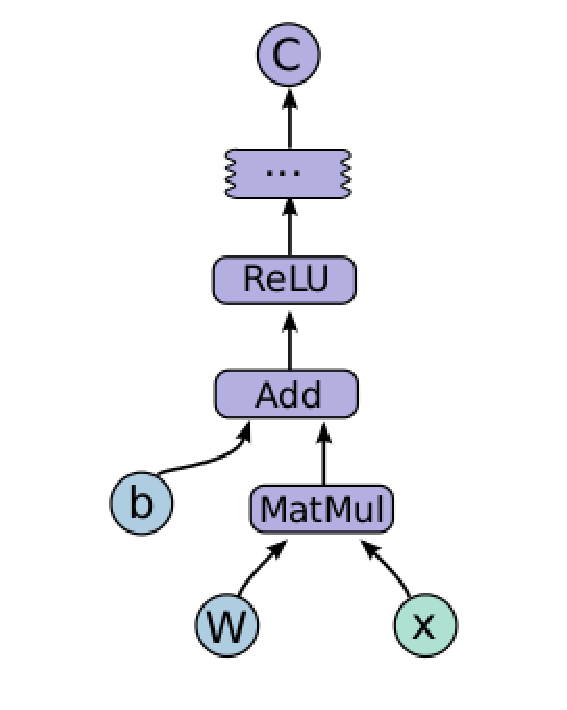
\includegraphics[width=4cm]{./img/tensorflow_graph.eps}
		\end{figure}
	\end{columns}
\end{frame}

\begin{frame}[fragile]
	\frametitle{TensorFlow computation graphs}
	\begin{columns}
	\column{0.68\textwidth}
		\begin{lstlisting}[style=Python]
import tensorflow as tf

b = tf.Variable(tf.zeros([100]))
W = tf.Variable(tf.random_uniform \
	([784,100],-1,1))
x = tf.placeholder(name="x")
relu = tf.nn.relu(tf.matmul(W, x) + b)
C = |[...]|

s = tf.Session()
for step in xrange(0, 10):
	x_in = |[...]| #construct 100-D input array
	result = s.run(C, feed_dict={x: x_in})
	print step, result
		\end{lstlisting}
	\column{0.28\textwidth}
		\vspace{-1.5cm}
		\hspace{-1cm}
		\begin{figure}
			\centering
			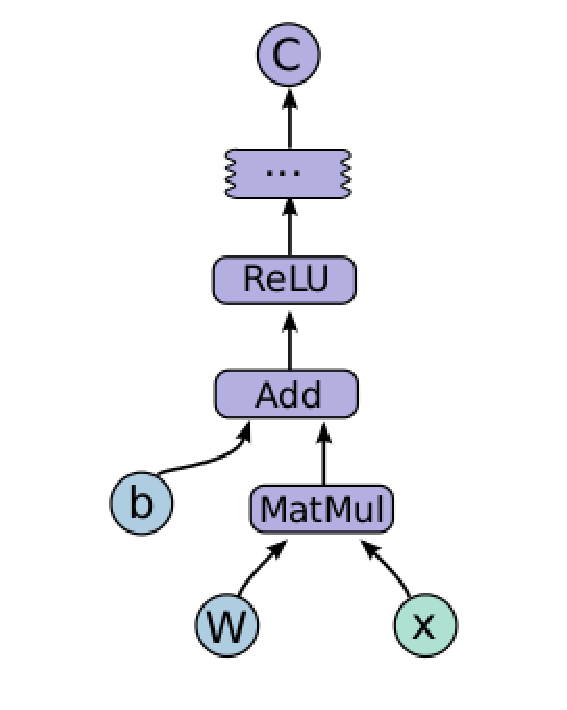
\includegraphics[width=4cm]{./img/tensorflow_graph.eps}
		\end{figure}
	\end{columns}
\end{frame}

% \begin{frame}
% 	\frametitle{NN with 2 hidden layer in TF}
% 	\begin{figure}
% 		\centering
% 		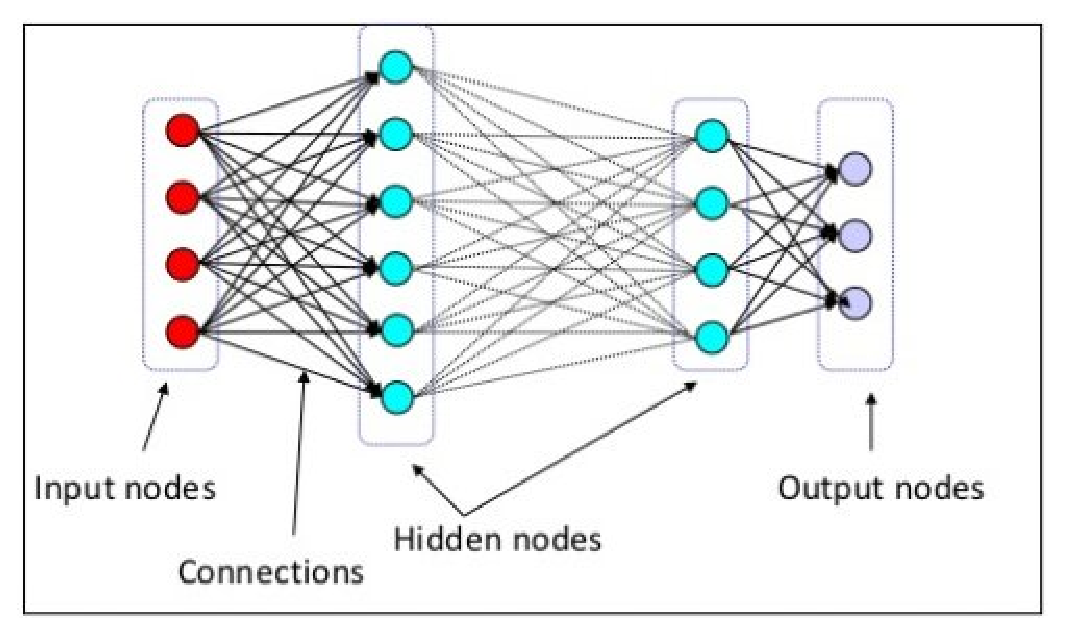
\includegraphics[height=4cm]{./img/neural-networks-layers.eps}
% 		\caption{\tiny{Source: \url{http://www.kdnuggets.com/2016/10/deep-learning-key-terms-explained.html}}}
% 	\end{figure}
% 	\begin{itemize}
% 		\item Implement such network is very easy in TF.
% 	\end{itemize}
% \end{frame}
% 
% \begin{frame}[fragile]
% 	\begin{lstlisting}[style=Python]
% def inference(images, n_hidden1, n_hidden2):
%   # Hidden 1
%   with tf.name_scope('hidden1'):
%     weights = tf.`Variable`(tf.`truncated_normal`([N_PIXELS, n_hidden1], |[...]|,name='weights')
%     biases = tf.`Variable`(tf.`zeros`([n_hidden1]), name='biases')
%     hidden1 = tf.nn.`relu`(tf.`matmul`(images, weights) + biases)
%   # Hidden 2
%   with tf.name_scope('hidden2'):
%     weights = tf.`Variable`(tf.`truncated_normal`([n_hidden1, n_hidden2], |[...]|, name='weights')
%     biases = tf.`Variable`(tf.`zeros`([n_hidden2]), name='biases')
%     hidden2 = tf.nn.`relu`(tf.`matmul`(hidden1, weights) + biases)
%   # Linear
%   with tf.name_scope('softmax_linear'):
%     weights = tf.`Variable`(tf.`truncated_normal`([n_hidden2, N_CLASSES], |[...]|, name='weights')
%     biases = tf.`Variable`(tf.`zeros`([N_CLASSES]), name='biases')
%     logits = tf.`add`(tf.`matmul`(hidden2, weights), biases, name = "logits")
%   return logits
% 	\end{lstlisting}
% \end{frame}

\begin{frame}[fragile]
	\frametitle{Brief list of some others TF features}
	\vspace{-0.15cm}
	\begin{itemize}
		\item Storing graphs and checkpoints into language neutral files (\texttt{protobuf} format).
		\pause
		\item Supports computation on CPU as well as on GPU, optionally supports CUDA.
% 		\begin{itemize}
% 			\item You can also specify where part of the code will run:
			\begin{lstlisting}[style=Python]
with tf.Session() as sess:
  with tf.device("/gpu:1"):
			\end{lstlisting}
% 			\item Will run on second GPU on given machine
% 		\end{itemize}
		\pause
		\item Can be run across the cluster, uses \texttt{grpc} for communication  
% 		\begin{itemize}
% 			\item uses \texttt{grpc} for communication 
% 			\item as simple as  ???????
			\begin{lstlisting}[style=Python]
with tf.device("/job:ps/task:0"):
  weights_1 = tf.Variable(...)
  biases_1 = tf.Variable(...)
|[...]|
with tf.device("/job:worker/task:7"):
  layer_1 = tf.nn.relu(tf.matmul(input, weights_1) + biases_1)
  logits = tf.nn.relu(tf.matmul(layer_1, weights_2) + biases_2)
|[...]|
with tf.Session("grpc://worker7.example.com:2222") as sess:
  sess.run(train_op)
			\end{lstlisting}
% 		\end{itemize}
	\end{itemize}
\end{frame}

\begin{frame}[fragile]
	\frametitle{TensorFlow integration with Infinispan/Java}
	\vspace{-0.1cm}
	\begin{itemize}
		\item Typically you create the model in Python and run it in C++ or Java app.
		\item TensorFlow Java API support still TBD, see TF \color{blue}\href{https://github.com/tensorflow/tensorflow/issues/5}{issue \#5}\color{black} and \color{blue}\href{https://github.com/tensorflow/tensorflow/issues/3}{issue \#3}\color{black}
		\item C++ API via JNI can be used as a workaround for Java.
		\item You can use some existing library, e.g. \color{blue}\href{https://github.com/bytedeco/javacpp-presets}{javacpp-presets}\color{black}.
	\end{itemize}
	\begin{lstlisting}[style=Java]
GraphDef graph = new GraphDef();
ReadBinaryProto(Env.Default(), modelPath, graph);
SessionOptions options = new SessionOptions();
this.session = new Session(options);
Status status = session.Create(graph);
|[...]|
Tensor img = new Tensor(DT_FLOAT, new TensorShape(1, image.length));
FloatBuffer imgBuff = img.createBuffer();
imgBuff.put(image);
|[...]|
TensorVector outputs = new TensorVector();
Status status = session.Run(new StringTensorPairVector(new String[] { "images" }, new Tensor[] { img }),
new StringVector("softmax_linear/logits"), new StringVector("softmax_linear/logits"), outputs);
	\end{lstlisting}
\end{frame}


\begin{frame}
	\frametitle{In-memory data grid: Infinispan}
	\begin{columns}
	\column{0.38\textwidth}
		\begin{figure}
			\centering
			
\includegraphics[width=3cm]{./img/infinispan.eps}
		\end{figure}
		\centering
		\vspace{0.3cm}
		\textbf{\color{blue}{\url{http://infinispan.org/}}}
	\column{0.6\textwidth}
		\begin{itemize}
			\item Data grid platform, written in Java
			\item In-memory No-SQL key-value data store, (optionally) schema-less
			\item Distributed cache - offers massive memory
			\item Elastic and scalable - can run on hundreds of nodes
			\item Highly available - no SPOF, resilient to node failures
			\item Transactional
			\item Supports indexing and searching
			\item Many other features
		\end{itemize}
	\end{columns}
\end{frame}

\begin{frame}[fragile]
	\frametitle{Infinispan eviction and cache stores}
	\begin{columns}
	\column{0.7\textwidth}
	\textbf{Eviction:} removing entries from the cache.
	\begin{lstlisting}[style=Java]
ConfigurationBuilder().eviction().size(|5|).strategy(EvictionStrategy.LRU)
	\end{lstlisting}
	\vspace{0.5cm}
	\textbf{Cache store:} a way how to store cache content in some external (persistent) storage.\\
	There are many, JDBC, JPA, clouds, LevelDB, Cassandra \dots and also \textbf{Ceph} cache store.
	\column{0.25\textwidth}
		\begin{figure}
			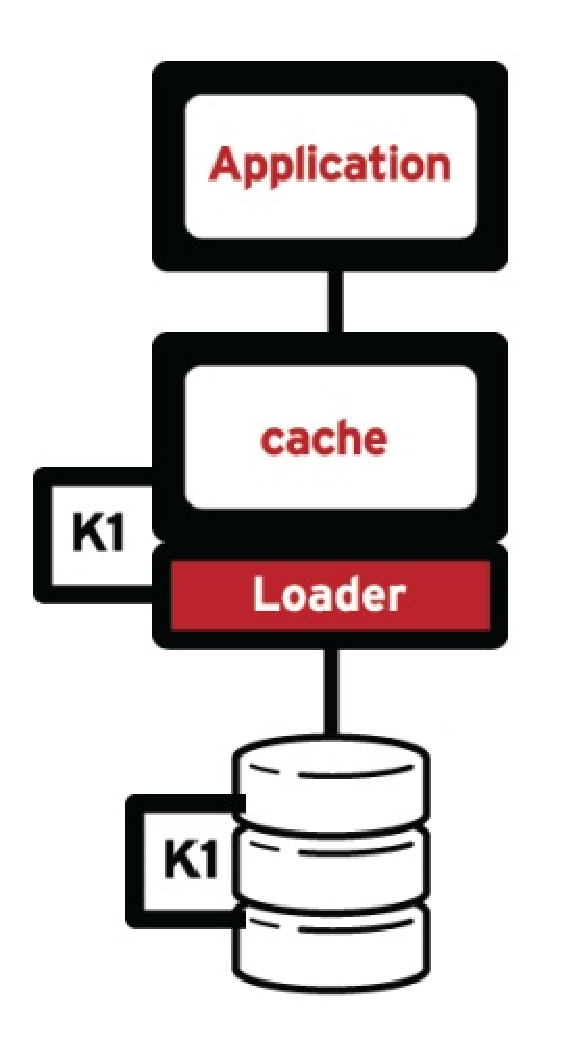
\includegraphics[width=3cm]{./img/cache_store.eps}
		\end{figure}
	\end{columns}
\end{frame}

\begin{frame}
	\frametitle{Ceph}
	\begin{columns}
	\column{0.38\textwidth}
		\begin{figure}
			\centering
			
\includegraphics[width=3cm]{./img/ceph_logo.eps}
		\end{figure}
		\centering
		\vspace{0.3cm}
		\textbf{\color{blue}{\url{http://ceph.com/}}}
	\column{0.6\textwidth}
		\begin{itemize}
			\item Distributed object storage.
			\item Provides interfaces to object, block and file system storage in unified data cluster.
			\item Scalable to the exabyte level.
			\item Highly available - no SPOF, resilient to node failures.
			\item Open source.
		\end{itemize}
	\end{columns}
\end{frame}

\begin{frame}[fragile]
	\frametitle{Ceph architecture and Infinispan cache store}
	\vspace{-0.5cm}
	\begin{columns}
	\column{0.4\textwidth}
	\begin{itemize}
		\item \texttt{rados} is distributed object store 
		%\item Apps can access \texttt{rados} directly via \texttt{librados} library.
		\item Infinispan cache store accesses \texttt{rados} directly via \texttt{librados} (using Java JNI client).
	\end{itemize}
	\column{0.6\textwidth}
		\begin{figure}
			\centering
			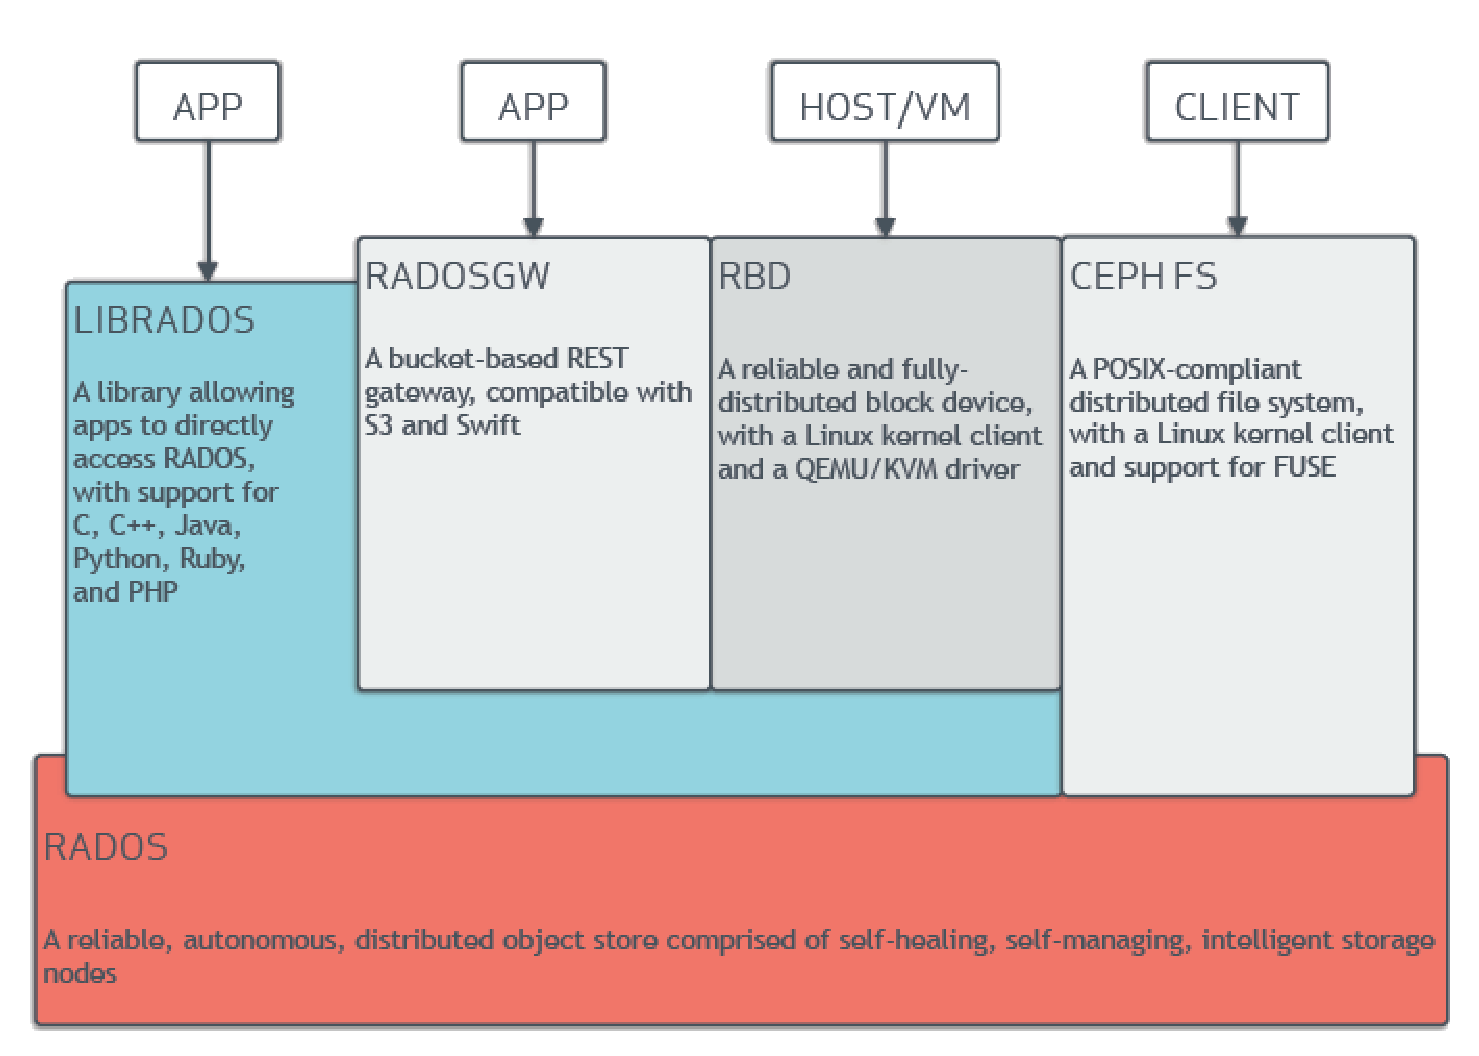
\includegraphics[width=6cm]{./img/ceph_arch.eps}
		\end{figure}
	\end{columns}
	\vspace{-0.3cm}
	Ceph cache store configuration:\\
	(details on \color{blue}\href{https://github.com/vjuranek/infinispan-cachestore-ceph}{https://github.com/vjuranek/infinispan-cachestore-ceph}\color{black}).
	\begin{lstlisting}[style=XML]
<local-cache name="cachestore" start="EAGER">
    `<store class="org.infinispan.persistence.ceph.CephStore">
        <property name="monitorHost">192.168.122.145:6789</property>
        <property name="userName">admin</property>
        <property name="key">mykey</property>
    </store>`
</local-cache>
	\end{lstlisting}
\end{frame}


\begin{frame}
	\frametitle{"Hello world" Demo}
	\centering
	Sources available on \textbf{\color{blue}{\url{https://github.com/vjuranek/tf-ispn-demo}}} \\
	\vspace{1cm}
	\Large\textbf{NN "Hello world" - MNIST data sample}
	\normalsize
	\vspace{0.5cm}
	\begin{itemize}
		\pause
		\item Recognition of hand written digits.
		\pause
		\item Besides simplicity, TF has very detailed tutorial for MNIST (for \color{blue}\href{https://www.tensorflow.org/tutorials/mnist/beginners/}{beginners}\color{black}~as 
		well as for \color{blue}\href{https://www.tensorflow.org/tutorials/mnist/pros/}{experts}\color{black})
	\end{itemize}
\end{frame}

\begin{frame}
	\frametitle{"Hello world" Demo}
	\begin{figure}
		\centering
		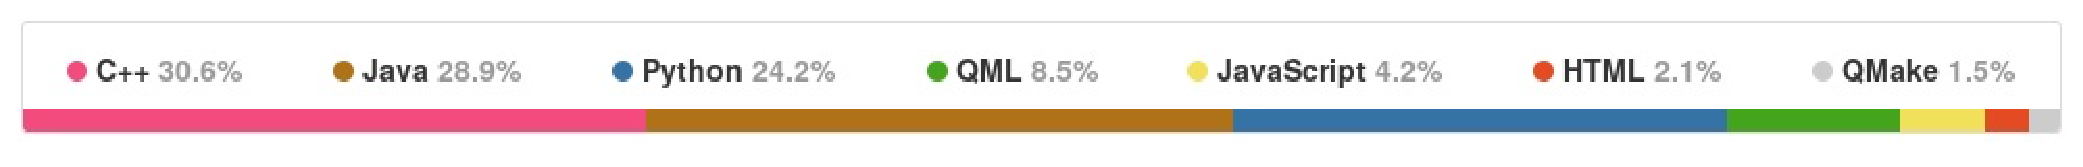
\includegraphics[width=12cm]{./img/demo_github.eps} \\
		\vspace{0.4cm}
		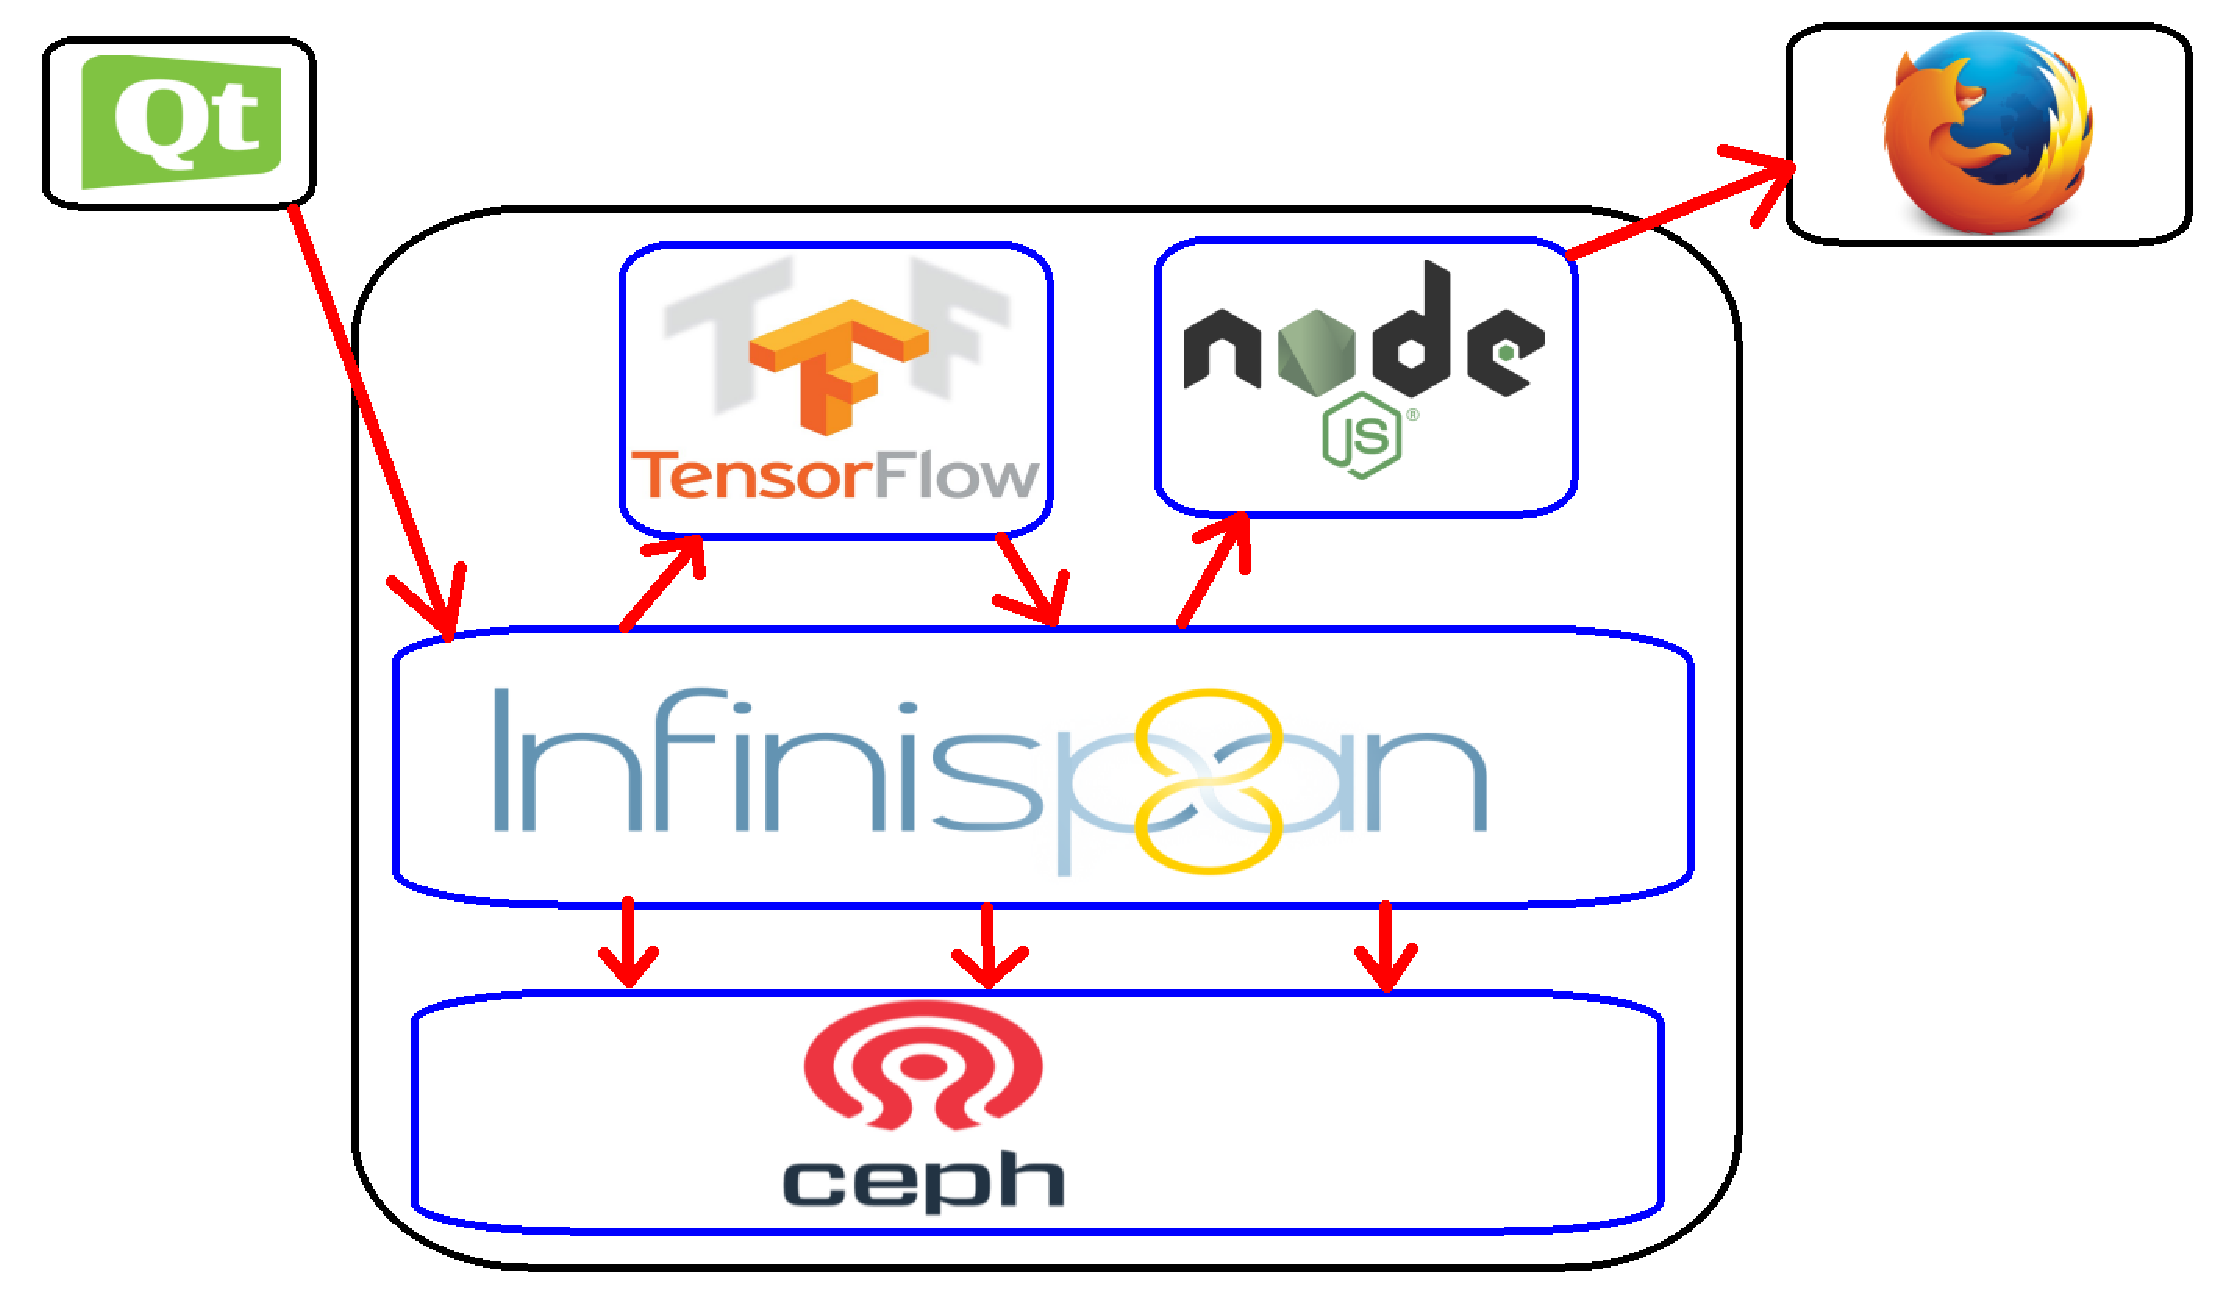
\includegraphics[width=12cm]{./img/demo_arch.eps}
	\end{figure}
\end{frame}

\begin{frame}
	\frametitle{Summary}
	\begin{itemize}
		\item Building pipeline for complex data processing in real time can be quite easy if you use the right tools.
		\pause
		\item TensorFlow is very powerful machine learning framework.
		\pause
		\item Infinispan is real middleware which can glue together various pieces of your application stack and server as its backbone.
	\end{itemize}
\end{frame}

\begin{frame}
	\frametitle{Question?}
	\begin{figure}
		\centering
		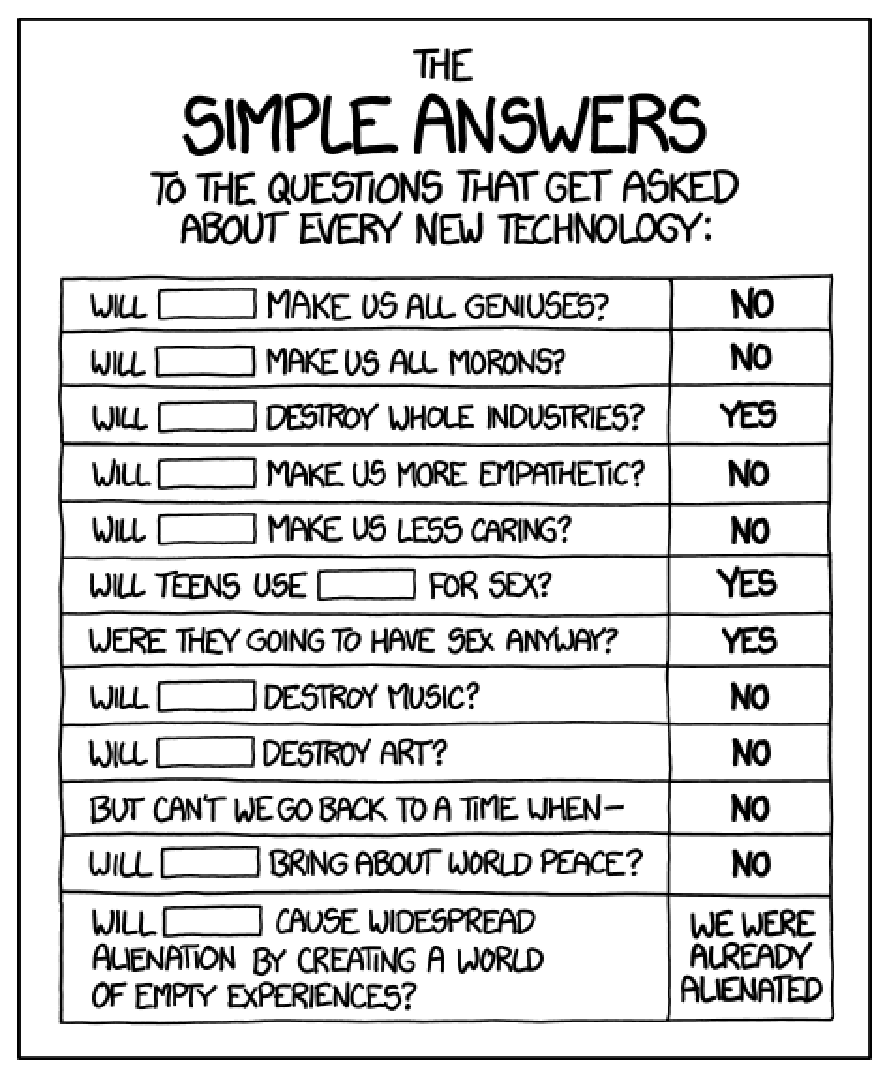
\includegraphics[width=6cm]{./img/simple_answers.eps}
		\caption{\tiny{Source: \url{https://xkcd.com/1289/}}}
	\end{figure}
\end{frame}

\begin{frame}
	\begin{figure}
		\centering
		
\includegraphics[width=5cm]{./img/infinispan8.eps}
	\end{figure}
	\centering
	\large{\color{blue}{\url{http://infinispan.org/}}} \\
	\vspace{1cm}
	\huge{\textbf{Thank you for your attention!}} \\
	%\vspace{1cm}
	%\huge{\textbf{Questions?}}
\end{frame}

\end{document}